%!TEX root = inversion.tex
%%%%%%%%%%%%%%%%%%%%%%%%%%%%%%%%%%%%%%%%%%%%%%%%%%%%%%%%%%%%%%%%%%%%%%%%%%%%%%
% Copyright (c) 2003-2018 by The University of Queensland
% http://www.uq.edu.au
%
% Primary Business: Queensland, Australia
% Licensed under the Apache License, version 2.0
% http://www.apache.org/licenses/LICENSE-2.0
%
% Development until 2012 by Earth Systems Science Computational Center (ESSCC)
% Development 2012-2013 by School of Earth Sciences
% Development from 2014 by Centre for Geoscience Computing (GeoComp)
%
%%%%%%%%%%%%%%%%%%%%%%%%%%%%%%%%%%%%%%%%%%%%%%%%%%%%%%%%%%%%%%%%%%%%%%%%%%%%%%

\chapter{DC Resistivity Forward modelling}\label{Chp:cook:Dc Resistivity inversion}
\section{Introduction}
DC resistivity surveys involve placing electrodes into the ground and injecting a current
into them. The current propagates through the ground and generates a potential field.
The change in potential between an other set of electrodes can then be measured.

As the separation between the electrodes increases, the current has a longer 
distance to travel and can potentially travel deeper. This is not necessarily the case 
as a highly conductive layer will keep the current close to the surface.

The final objective is to perform an inversion and develop a resistivity image of the subsurface.
This image can then be compared to known resistivities of material and used 
to make inferences about the material contained in the subsurface.
There are a number of different ways to set up a DC resistivity survey, each providing
different spatial information\cite[pg 5]{LOKE2014}.

Escript currently supports the forward modelling of DC resistivity surveys. Forward modelling
involves performing a survey artificially by solving the PDEs which describe the underlying
physics. Escript provides a number of classes for solving forward modelling problems, these are
detailed in section \ref{sec:forward DCRES}.

\section{Example}
In this section we will look at an example forward problem. The domain consists of
a homogeneous half-space with a half-sphere embedded within it (Figure~\ref{fig:HalfSphere}). 
In this example\footnote{The script is similar to
\examplefile{dc_forward.py} within the \escript example file directory.}
 a Schlumberger survey is used.


\begin{figure}
\centering
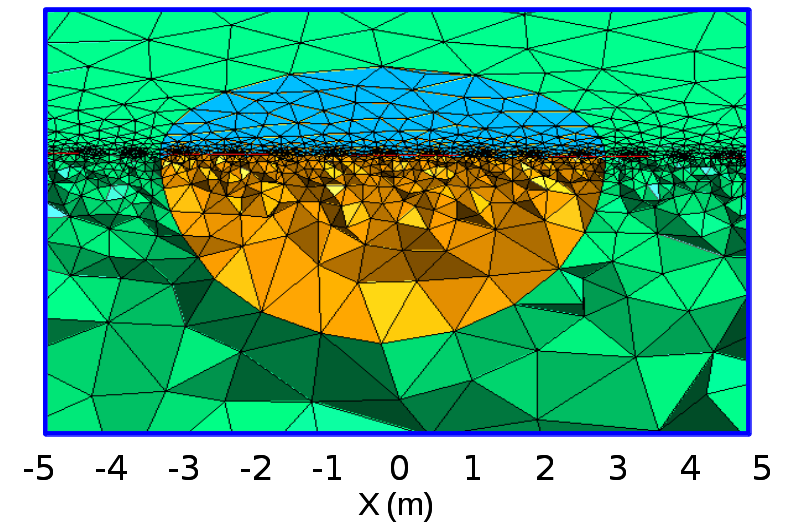
\includegraphics[width=0.7\textwidth]{HalfSphere.png}
\caption{
    (file \examplefile{data/HalfSphere_v1.4.geo}). model created using gmsh.}
\label{fig:HalfSphere}
\end{figure}

\begin{pyc}\label{code: dc1}
\
\begin{python}
#Header
import esys.finley      as finley
import esys.escript     as escript
from esys.downunder     import *
import math

#Constants
pi = math.pi

#Setup Input
mesh_file = "data/HalfSphere_v1.4.msh"
# Tag volume names and conductivity values (S/m) for primary 
# and secondary potential:
tag_p = {"domain" : 1/10.0, "sphere" :  1/10.0} # Primary (homogeneous).
tag_s = {"domain" : 1/10.0, "sphere" :  1/1.0 } # Secondary.

xe_0 = -5.0 # start X-coordinate
numEle =  21  # number of electrodes
a =  0.5 # step size
n = 9 #max electrode step
midPoint = [xe_0 + (((numEle-1)*estp)/2), 0, 0]
current = 1.0 # (Ampere)
domain = finley.ReadGmsh(mesh_file, 3)
mesh_tags = escript.getTagNames(domain)
directionVector = [1,0]
sig_p = escript.Scalar(0,escript.ContinuousFunction(domain))
sig_s = escript.Scalar(0,escript.ContinuousFunction(domain))
for tag in tag_p:
    # All initially defined tags must be in the tag list.
    # Print an error if it doesn't and exit the program.
    if tag in mesh_tags:
        # Assign value:
        sig_p.setTaggedValue( tag, tag_p[tag] )
        sig_s.setTaggedValue( tag, tag_s[tag] )
    else:
        print("Error: the defined tag is not defined in the mesh: " & tag)
        sys.exit()

# Expand the data objects for output.
sig_p.expand()
sig_s.expand()
#solve for result
schs=SchlumbergerSurvey(domain, sig_p, sig_s, current, a, n, midPoint, 
    directionVector, numEle)
pot=schs.getPotential()
totalApparentRes=schs.getApparentResistivityTotal()
#print result
n=1
print ("Total:\n")
for i in totalApparentRes:
    print ("n = %d:"%n)
    print (i,"\n")
    n=n+1
\end{python}
\end{pyc}


The example begins with constructing the domain, loaded from a pre-prepared
\emph{gmsh} model. The \emph{gmsh} script used can be found in \examplefile{data/HalfSphere_v1.4.geo}.
\emph{gmsh} can be used to generate the \texttt{msh} file. The values for primary and secondary 
conductivity, in Siemens per meter, are specified for the different regions. These regions have been tagged
in the \emph{gmsh} script. The survey is constructed to have 21 electrodes spanning from -5m to 5m
in the $x$-axis, with a fixed interval between each electrode and the next in 
line. These electrodes, once placed, are not moved for the remainder of the
survey. The potentials and total apparent resistivity is then calculated.

The SchlumbergerSurvey class uses four electrodes at a time, beginning with the
electrode at location \texttt{xe_0}. In each set of four electrodes, electrodes
1 and 4 are used as current electrodes and 
2 and 3 used as potential electrodes. The next set of electrodes are then used
for the next measurement, beginning with the previous electrode 2. This is 
repeated until the last four electrodes are used.

This process is itself repeated with a continually increasing step size between
the electrodes pairs at each end of the set. As an example, the first time the
process is repeated, the initial set will be made up of electrodes 1, 3, 4, and
6. During the second repeat the initial set will be electrodes 1, 4, 5, and 8.
The maximal step size in the above script is given as $n$.
 
